\documentclass{report}

\usepackage[utf8]{inputenc}
\usepackage[T1]{fontenc}
\usepackage[francais]{babel}
%\usepackage{layout}
%\usepackage{geometry}
%\usepackage{setspace}
\usepackage{soul}
\usepackage{ulem}
%\usepackage{eurosym}
%\usepackage{bookman}
%\usepackage{charter}
%\usepackage{newcent}
%\usepackage{lmodern}
%\usepackage{mathpazo}
%\usepackage{mathptmx}
%\usepackage{url}
%\usepackage{verbatim}
%\usepackage{moreverb}
%\usepackage{listings}
%\usepackage{fancyhdr}
\usepackage{wrapfig}
\usepackage{graphicx}
%\usepackage{color}
\usepackage{xcolor}
%\usepackage{colortbl}
\usepackage{amsmath}
\usepackage{amssymb}
\usepackage{mathrsfs}
%\usepackage{asmthm}
%\usepackage{makeidx}
\usepackage{float}


\title{Système autonome pour le traitement et l'exploitation de données GPS}
\author{COUNOT Thibaut et WARTELLE Adrien}
\date{13/06/17}

\begin{document}

\maketitle
\tableofcontents

\chapter{Introduction}
\section{Présenation du groupe}
Nous sommes deux étudiants en branche ingénieur à l'UTT :
un en branche A2I 2 (Thibaut) et l'autre en RT 3 (Adrien en filière TMSE). 
Nous avons choisi l'unité d'enseignement IF23 sur la géolocalisation 
principalement parce qu'elle traite 
de problématiques d'informatique embarquée et modélisation mathématique
pour le traitement de données. Nous sommes en effet intrigués par le
fonctionnement de l'informatique au plus bas niveau, ce sur quoi repose
toutes les technologies modernes.

\section{Cahier des charges}

Dans le cadre de cette unité d'enseigement, nous avons du réaliser
un mini-projet GPS dont l'objectif a été de programmer un SOC (Système
 On Chip) Arduino pour lui permettre de manipuler, d'afficher et 
 d'enregistrer des données satellites. Notre travail s'est décomposé
 en deux parties :
 \begin{itemize}
 \item Programmation du système GPS
 \item Traitement et exploitation des données enregistrées
 \end{itemize}
 En effet, nous avons du programmer un système embarquée
 avec toutes les problématiques d'optimisation en incorporant des
 fonctionnalités pour l'affichage de l'autonomie, des coordonées
 pour l'enregistrement (horodatage, choix durée d'enregistrment
 et d'intervalle) et la transmission des données. \\
 De plus, nous avons du effectuer un traitement des données enregistrées
 à l'aide du SOC comme la transformation de coordonnées dans différents
 repéres (cartésien et local depuis géocentrique). Nous avons testé
 différents protocoles de parcours pour étudier différents phénomènes
 à l'aide d'indicateurs statistiques (moyenne, variance, corrélation). 

\section{Outils et resources}
La programmation du système GPS a necessité de multiples composants
électroniques : une carte Arduino équipé d'une ATmega328 (8bits, 3.3V,
32ko de Flash et 2ko SRAM), d'une carte SD, d'un écran LCD, d'un boitier
muni de boutons, d'un récepteur GPS et d'interfaces séries pour la 
communication entre les composants. Pour programmer le système GPS, nous
avons utilisé l'environnement de développement d'Arduino qui permet de
compiler du code C/C++ pour un processeur AVR (à l'aide d'avrgcc) et nous
nous sommes servi de Git et d'un fichier TODOLIST
 pour la gestion du projet que l'on peut retrouver
à l'adresse suivante : \\
https://github.com/Adrilord/GogolPS \\

Le traitement des données a nécessité l'intervention du logiciel Matlab
et d'Octave (version libre GNU)
pour effectuer les calculs rapidement et facilement. Nous avons aussi
utilisé un petit programme pour transformer le format des données brut
en un format KML pour la visualisation.

Nous avons eu de nombreux problèmes avec les composants GPS : 3 problèmes
de déchargement des piles, un problème persistant de carte SD ainsi qu'un
problème d'espace mémoire pour l'enregistrement et la transmission des
données provoqué par le faite que la librairie SD d'Arduino occupe plus
de 50\% des 2ko disponibles en SRAM. Ces multiples problèmes nous
ont fait perdre plusieurs semaines (au moins 3) et nous ont obligés à changer
2 fois de boitiers et à réécrire entièrement 2 fois le programme GPS. 
Ainsi nous n'avons eu au final que quelques jours pour nous occuper
du traitement des données que nous aurions voulu plus approfondir.

\chapter{Programmation du système GPS}
\section{Démarche}
La programmation du système GPS s'est effectué en 4 étapes :
\begin{itemize}
 \item Tests matériels
 \item Tests de modélisation sur ordinateur en C++
 \item implémentation 1 
 \item implémentation 2 finale
 \end{itemize}
Nous avons effectué de nombreux Tests avant de pouvoir commencer
à implémenter réellement le programme sur Arduino. Nosu avons en effet
écris (et repris) 4 tests matériels (dans Tests/testsMatériel) pour la carte SD
le module GPS, les piles et les boutons. 
Une fois que cela effectué nous avons commencé à modéliser notre 
programme en utilisant le patron de conception MVC : Modèle Vue Contrôleur.

Le modèle contient toutes les données du programme qui nous intéressent
avec des données locales avec l'autonomie, les paramètres de temps de parcours
 et toutes les données que l'on peut recevoir depuis le gps. Ce modèle
 est mis à jour régulièrement pour avoir une version actualisée
 (récente) des données que l'on affiche ou enregistre. \\
 
Les vues sont tous simplement les menus à afficher. Ils contiennent
les informations d'affichage pour les cases du LCD et des informations
sur sa configuration et sa configurabilité. Nous avons initialement 
modélisé les menus comme ceci (SW étant les switchs qui permmettent
la transition entre les menus) :

\begin{figure}[H]
	\begin{center}
		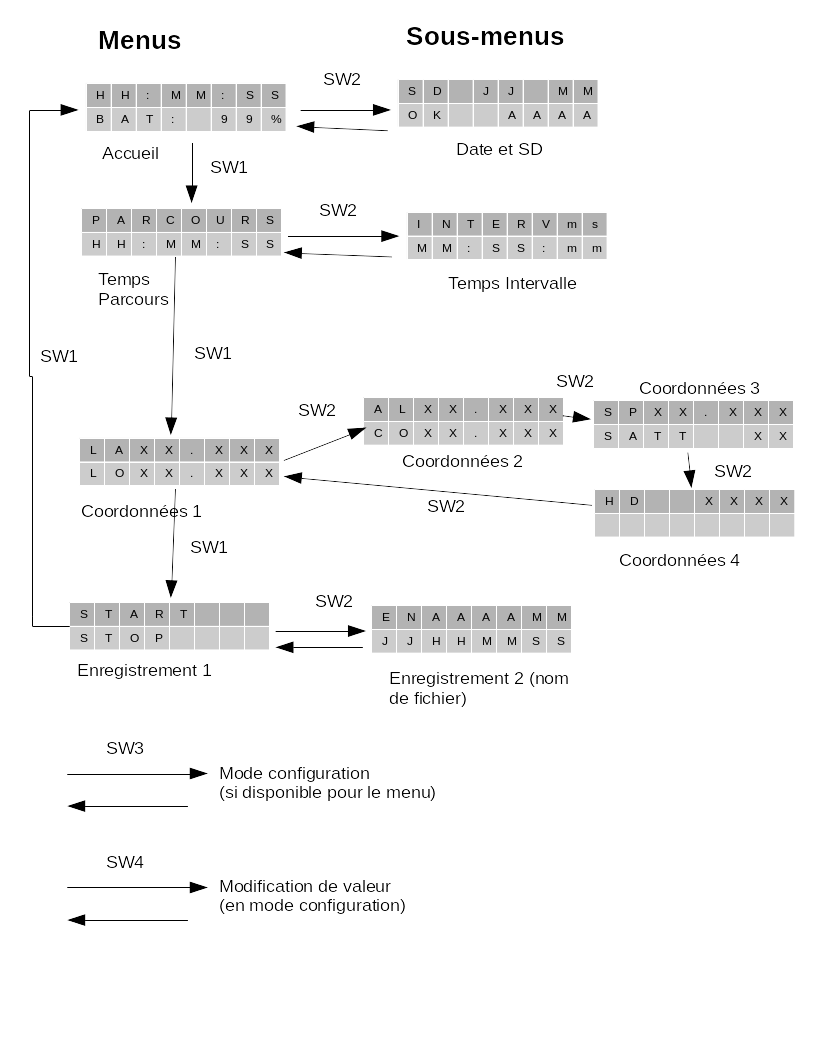
\includegraphics[scale=0.5]{diagrammeCasUtilisation1.png}
	\end{center}
	\caption{Diagramme d'utilisation initial du système}
\end{figure}

Nous n'savons pas implémenté un contrôleur à proprement parlé, nous avons
utilisé différents modules à la place qui permettent de manipulé le
modèle et les menus.

Après avoir modélisé notre système, nous l'avons implémenté en C++ (dans Tests/testsCpp) en
utilisant un terminal et le clavier au lieu du système arduino avec lcd
et boutons. Nous nous sommes rapidement rendus compte que la 
programmation orientée objet allait
être lourde et allait imposer une syntaxe difficile tout en nous empêchant
d'optimiser le programme. Nous avons alors réimplémenter cela en C (dans Tests/testC) en
utilisant des structure et des fonctions sur celles-ci. \\
Au moment de transférer le code sur l'arduino, nous avons réalisé que
les fonctions de la librarie standarde de C pour la manipulation des
caractères que nous devions faire n'allait pas être possible (trop de place
prise). Nous avons ainsi reprogrammé des fonctions basiques pour manipuler
les chaines de caractère.

En intégrant la solution dans l'Arduino avec l'implémentation 1, 
nous nous sommes rendus compte
que, même après avoir optimisé au mieux l'utilisation de la mémoire, il
manquait encore de la mémoire pour pouvoir enregistrer et transférer les
données.

Nous avons alors encore une fois réécrit une implémentation en simplifiant
au maximum le programme : en mettant tout dans le même programme, en
 utilisant uniquement des variables simples (pas de structure), en
 simplifiant au maximum les menus (suppression des sous-menus)
 et ne gardant que les fonctionnalités essentielles. 
 Nous sommes aboutis à ce diagramme :
 
\begin{figure}[H]
	\begin{center}
		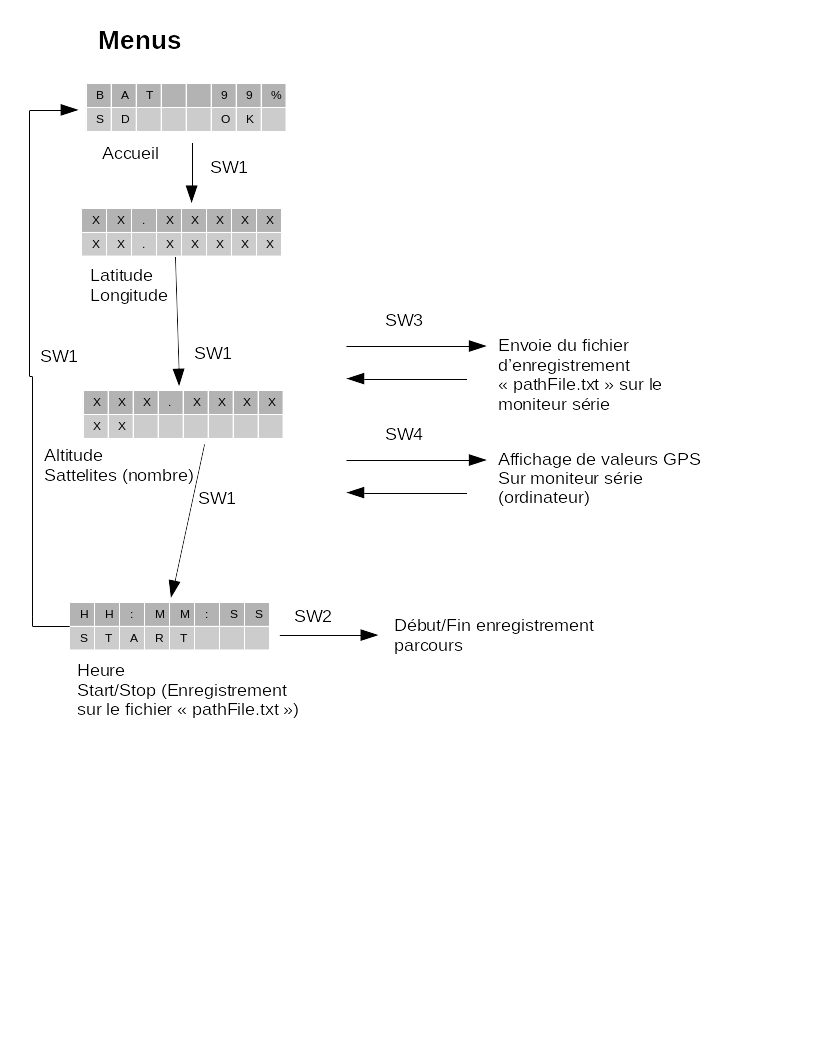
\includegraphics[scale=0.5]{diagrammeCasUtilisation2.png}
	\end{center}
	\caption{Diagramme d'utilisation final du système}
\end{figure}

C'est grâce à cette dernière implémentation que nous avons pu effectuer
ls parcours.
 

\section{Modèle MVC et implémentation 1}

La première implémentation sur Arduino est constitué de 6 modules :
\begin{itemize}
\item implemArduino
\item charmanagment
\item datetime
\item iomanagement
\item menu
\item model
\end{itemize}

Le module model contient une structure décrivant le modèle
sous format nombre et une sous format caractères (ASCII). Il contient
aussi des fonctions d'initialisations et mis à jour et de
transformation (format nombre au format caractères). \\
Le module menu contient une structure décrivant un menu avec ses
variables pour la gestion de la configuration (groupe d'id notamment),
et les types de menu auquel il est connecté par SW1 et SW2. Il contient
aussi des fonctions pour l'affichage (pour le lcd), la génération de menu
à partir de son type, la mise à jour du contenu d'un menu et des 
fonctions pour la gestion de la configuration. \\
Le module charmanagement implémente des fonctions simples pour la
manipulation de chaînes de caractères et pour la transformation de
nombres en chaînes de caractères. \\
Le module datetime contient une structure permettant de représenter 
une date avec le temps. On y trouve une fonction d'initialisation.

Le module iomanagement contient une struture pour la configuration
de l'enregistrement d'un parcours. Ce module est partiellement
implémenté car c'est à ce moment que nous nous sommes rendus
compte des problèmes de mémoire. On y trouve des fonctions pour
initialiser la configuration d'enregistrement et des fonctions
pour l'enregistrement des données et des paramètres de temps de parcours.

Finalement le module implemArduino contient le programme principal
que l'on peut résumer par le schéma suivant :

\begin{figure}[H]
	\begin{center}
		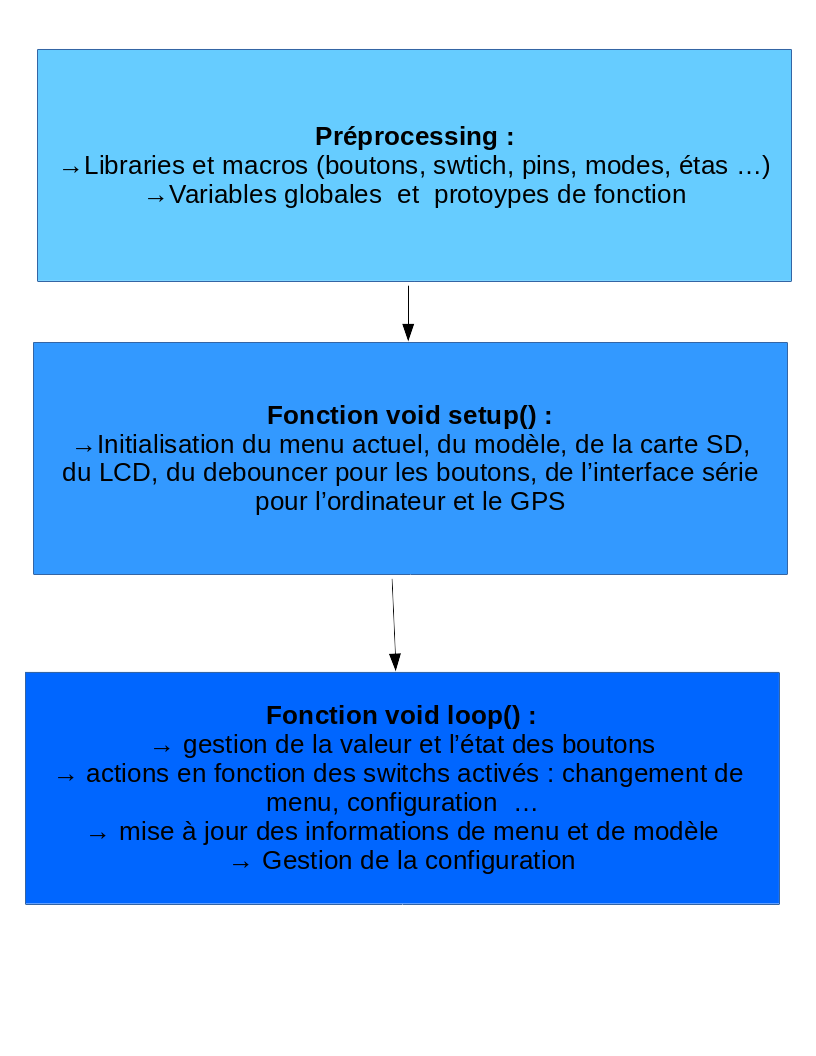
\includegraphics[scale=0.5]{schemaProgramme.png}
	\end{center}
	\caption{Schéma du programme principal}
\end{figure}

Après la fonction loop, on trouve des fonctions pour la gestion des
des boutons, un délai intelligent pour le GPS qui intègre l'encodage
des données, pour des tests éventuels.

La gestion des boutons consiste à détecter des changements de valeur
des pins, on change alors les états des boutons (attention ce que l'on
appel bouton ici correspond à un signal reçu sur l'arduino et non
à un switch (vraie bouton) du boitier) et en fonction
de la combinaison d'états, on sait quel switch a été activé.

Cette première implémentation permettait de remplir toutes les
fonctionnalités du cahier des charges à l'exception de l'enregistrement.
Nous avons donc mis en place rapidement (il restait de 2 semaines)
une seconde implémentation.

\section{Modèle Simple et implémentation 2}

Cette implémentation reprend le programme principal de la première
implémentation tout en intégrant l'affichage et la mise à jour des 
menus et des données de modèle directement dans le code notamment
avec des variables globales simples. On a enlevé la gestion de la
configuration, la gestion des paramètres, simplifié le système de menu.
Nous avons décidé d'utiliser un unique fichier pour l'enregistrement des
parcours ("pathFile.txt") que l'on réécrit à chaque enregistrement. L'intervalle
d'enregistrement est de 5 secondes et on enregistre avec le start/stop
(switch SW3). Il faut enregistrer les donnés du parcours précédent
sur ordinateur (grâce à une transmission série) avant de pouvoir
commencer une nouvelle.

Nous avons fait ces choix de simplification pour s'assurer d'avoir
 suffisament de mémoire pour l'enregistrement et donc pour pouvoir rapidement commencer la partie traitement.



\chapter{Traitement et exploitation des données enregistrées}
\section{Protocoles des parcours}
Nous avons effectué trois parcours : un immobile sous un toit (fichier
"enrUno1206"), un mobile autour du parking devant le laboratoire X de
l'UTT en passant sous des arbres (fichier "enrDos1206") et un immobile à l'air libre sans grand obstacle devant le foyer étudiant (fichier 
"enrTres1206").
Tous ces enregistrements ont été effectués le 12/06/17 au format "brut"
où les valeurs de GPS sont juste séparés par des virgules sur une ligne
et chaque ligne correspond à un enregistrement (les enregistrements
étant séparés de 5 secondes).
\section{Visualisation KML}
\section{Traitement matlab}
\section{Résultats}

\chapter{Conclusion}

\end{document}
